\documentclass[11pt,a4paper,english]{article}
\usepackage[english]{babel} % Using babel for hyphenation
\usepackage{lmodern} % Changing the font
\usepackage[utf8]{inputenc}
\usepackage[T1]{fontenc}

\usepackage[colorlinks=true]{hyperref}

%\usepackage[moderate]{savetrees} % [subtle/moderate/extreme] really compact writing
\usepackage{tcolorbox}
\tcbuselibrary{hooks}
\usepackage[parfill]{parskip} % Removes indents
\usepackage{amsmath} % Environment, symbols etc...
\usepackage{amssymb}
\usepackage{float} % Fixing figure locations
\usepackage{multirow} % For nice tables
%\usepackage{wasysym} % Astrological symbols
\usepackage{graphicx} % For pictures etc...
\usepackage{enumitem} % Points/lists
\usepackage{physics} % Typesetting of mathematical physics examples: 
                     % \bra{}, \ket{}, expval{}
\usepackage{url}

\definecolor{red}{RGB}{255,10,10}

% To include code(-snippets) with æøå
\usepackage{listings}
\lstset{
language=c++,
showspaces=false,
showstringspaces=false,
frame=l,
}

\tolerance = 5000 % Bedre tekst
\hbadness = \tolerance
\pretolerance = 2000

\numberwithin{equation}{section}

\newcommand{\conj}[1]{#1^*}
\newcommand{\ve}[1]{\mathbf{#1}} % Vektorer i bold
\let\oldhat\hat
\renewcommand{\hat}[1]{\oldhat{#1}}
\newcommand{\trans}[1]{#1^\top}
\newcommand{\herm}[1]{#1^\dagger}

\newcommand{\Real}{\mathbb{R}}
\newcommand{\bigO}[1]{\mathcal{O}\left( #1 \right)}

\newcommand{\di}{\mathrm{d}}
\newcommand{\magM}{\mathcal{M}}

\newcounter{algcounter}
\renewcommand{\thealgcounter}{\Roman{algcounter}}

\newenvironment{algorithm}{%
\refstepcounter{algcounter}
\begin{tcolorbox}
\centerline{Algorithm \thealgcounter}\vspace{2mm}
}
{\end{tcolorbox}}

\newcommand{\figurewidth}{.85\textwidth}

\title{FYS3150/4150\\Computational Physics\\Project 4}
\author{Candidate numbers ?? and ??}
\date{\today}

\begin{document}
\tcbset{before app=\parfillskip0pt}
\maketitle

\begin{abstract}
This project explores the Ising model applied to spins in two dimensions.
\end{abstract}



\section{Introduction}


\section{Theory}

The energy of a spin system in the Ising model 
\begin{gather}
E = -J\sum_{\expval{kl}}^N s_k s_l
\end{gather}
Since only pairwise interactions are counted, this can be rewritten to
\begin{gather}
E = -J\sum_{k\expval{l}} s_k s_l = -J \sum_{k} s_k s_{k+1}
\end{gather}



With $s_i = \pm 1$, N number of spins, J coupling constant, summed over 
the closest neighbours only. This leads to a boundary problem, which 
can be solved in multiple ways. In our model we are 
using periodic boundary conditions,
\begin{gather}
s_k = s_{k \pm L}
\label{eq:boundary}
\end{gather}
An illustration of this is visible in figure \ref{fig:spin_neighbours}.

\begin{figure}[H]
\centering
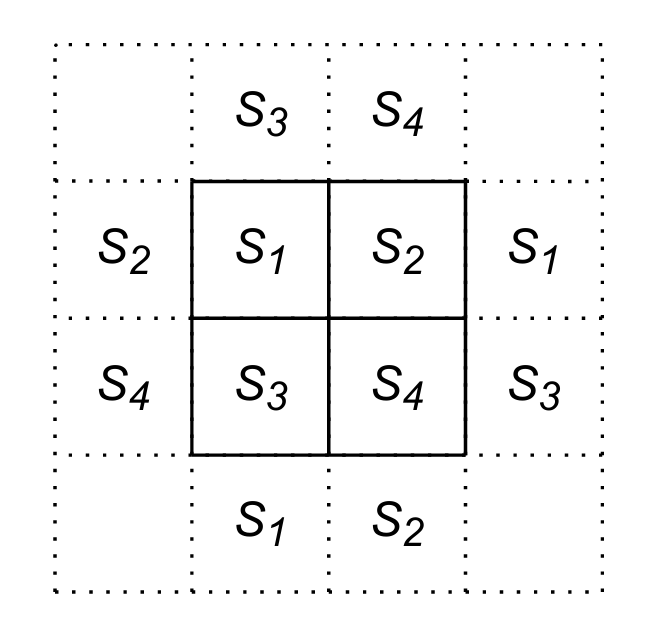
\includegraphics[scale=0.15]{pics/simple_lattice.png}
\caption{ Illustration of the simple, ''$L=2$''-lattice and a graphical interpretation the periodic boundary conditions.}
\label{fig:spin_neighbours}
\end{figure}

\subsection{Statistical mechanics}
The partition function
\begin{gather}
Z = \sum_i \exp(-\beta E_i)
\end{gather}

\subsubsection{Energy}

\begin{gather}
\expval{E} = -\frac{\partial Z}{\partial \beta}
\end{gather}


\subsubsection{Magnetisation}
From partition function
\begin{gather}
\expval{\magM} = \frac{p(\magM_i)}{Z}
\end{gather}

The net magnetisation is defined by
\begin{gather}
\magM = \sum_k s_k
\end{gather}
There should be a critical temperature where this one flips from 
zero to some value for ferromagnets (positive J)

\subsubsection{Spesific heat}
\begin{gather}
C_v = -\frac{\partial \expval{E}}{\partial \beta}
 = \frac{\partial^2 \ln Z}{\partial \beta^2}
\end{gather}

\subsubsection{Susceptibility}
\begin{gather}
\chi = \frac{\partial\expval{\magM}}{\partial \beta}
\end{gather}



\subsection{Simple system}
For the simple case of only two spins in each dimension($L=2$)
the energies are summed by
\begin{gather}
E = -J\sum_{x,y}^{L} s_x (s_{x+1,y} + s_{x,y+1})
\end{gather}
The energy is then a function of the spins,
\begin{equation}
E = -2J(s_1s_2 + s_1s_3 + s_2s_4 + s_3s_4)
\end{equation}
This has symmetries with regards to which spin is up.
Listing up all the different spin configurations, their degeneracy 
and the energies,
\begin{gather*}
\text{Spin configuration} = 
\begin{cases}
n_{up} = 0, \quad d=1, \quad E = -8J\\
n_{up} = 1, \quad d=4, \quad E = 0\\
n_{up} = 2, \quad d=6, \quad 
\begin{cases} 
\text{diag} \quad d = 2, \quad E = 8J\\
\text{non-diag} \quad d = 4, \quad E = 0
\end{cases}\\
n_{up} = 3, \quad d=4, \quad E = 0\\
n_{up} = 4, \quad d=1, \quad E = -8J
\end{cases}
\end{gather*}
The energies with their degeneracy is then
\begin{gather}
E = 
\begin{cases}
-8J, \quad d = 2\\
\phantom{-}0, \quad\quad d = 12\\
\phantom{-}8J, \quad d = 2
\end{cases}
\end{gather}
And the (absolute) magnetisation is
\begin{gather}
\abs{\magM} = 
\begin{cases}
4, \quad d = 2,\quad E = -8J\\
2, \quad d = 8, \quad E = 0\\
0, \quad
\begin{cases}
d = 2, \quad E = 8J\\
d = 4, \quad E = 0
\end{cases}
\end{cases}
\end{gather}
The partition function
\begin{gather}
Z = \sum_i d(i) e^{-E_i\beta} = 2e^{+8J\beta}+12e^{0}+2e^{-8J\beta}
 = 12 + 4\cosh(8J\beta)
\end{gather}
% This expression is expandened to the low energy case and the 
% high temperature case.
% \begin{gather}
% \expval{E}_{\beta\to\infty} = -8J\\
% \expval{E}_{\beta\to0} = \frac{64}{3}J^2\beta
% \end{gather}
% \begin{gather}
% C_{v,{\beta\to\infty}} = 0\\
% C_{v,\beta\to0} = \frac{128}{3}J^2
% \end{gather}
% Magnetism
% \begin{gather}
% \expval{\abs{\magM}} = \frac{4\cdot2e^{8J\beta} + 2\cdot 8e^{0} + 
% 0\cdot (2e^{-8J\beta} + 4e^{0})}{Z}\\
% \expval{\abs{\magM}}_{\beta\to\infty} = 4
% \end{gather}




\subsection{Analytical solutions}

\textcolor{red}{KSK: Maybe make this section consistent with the notation of $\beta = 1/ k_B T$ ? And add reference for 2D. solution}

\subsubsection{1-D Ising model}
Solutions for the Ising model in one dimension for a very large number of particles are known(Plischke and Bergersen, 1994). 

\begin{equation}
\frac{U}{J} = -N \tanh \left( \frac{J}{k_B T} \right) = -N \frac{e^{J/k_B T}-e^{-J/k_B T} }{e^{J/k_B T}+ e^{-J/k_B T} } =  \begin{cases} N, \quad k_B T \to 0 \\ 0, \quad  k_B T \to \infty \end{cases}
\end{equation}

The specific heat per particle and the magnetisation are given by 

\begin{equation}
C(T) = \frac{1}{N} \frac{dU}{dT} = \frac{(J/k_B T)^2}{cosh^2 (J/k_B T)}
\end{equation}
\begin{equation}
\magM(T) = \frac{N e^{J / k_B T} sinh(B/k_B T) }{ \sqrt{ e^{2J/k_B T} sinh^2 (B/k_B T) + e^{-2J/ k_B T}  } }
\end{equation}

\subsubsection{2-D Ising model}
There are known analytical solution to the two dimensional model as well, 

\begin{equation}
\magM (T) = \begin{cases} 0, \quad T > T_C \\ \frac{(1+z^2)^{1/4} (1-6z^2 + z^4 )^{1/8} }{(1-z^2)^{1/2}}, \quad T < T_C \end{cases}
\end{equation}
\begin{equation}
k T_C/J = \frac{2}{\ln(1+ \sqrt{2}) } \approx 2.269
\end{equation}

here $T_C$ is the \emph{Curie temperature} and $z = e^{-2J/k_B T}$. 

\section{Implementation}

A lattice class with periodic boundary conditions, so access of an
element follows \eqref{eq:boundary}. The energy of an element in the 
lattice and the total energy is easily calculated from the definition
of the energy. 

\subsection{The metropolis algorithm}

The probability of transition from i to j 
is modeled by the Boltzmann coefficient
\begin{gather}
w_j = \exp(-\beta (E_i - E_j))
\end{gather}
This suggest the following probabilities for moving to this state:
\begin{gather}
p = \begin{cases}
1 \quad\text{ if }  E_i - E_j \le 0\\
\exp(-\beta \Delta E) \text{ else}
\end{cases}
\label{eq:transition}
\end{gather}
This probability is compared with a random number generated from 
the computer.

For our lattices the factor $\Delta E$ is rather simple. Considering 
a case with one spin $s_0$ surrounded by $s_1,s_2,s_3, s_4$. 

\begin{figure}[H]
\centering
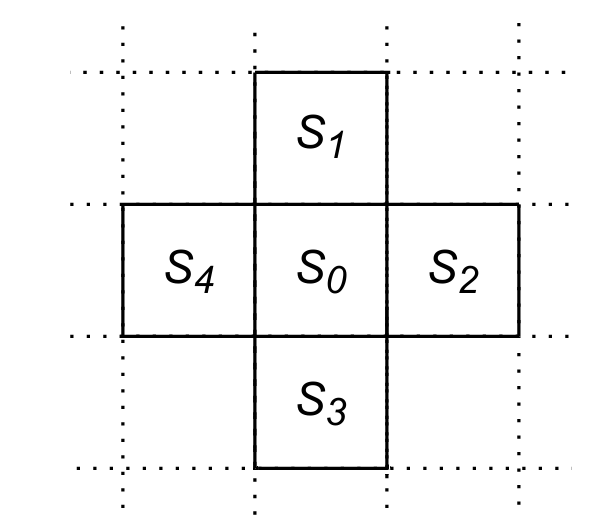
\includegraphics[scale=0.2]{pics/full_lattice.png}
\caption{ Illustration of $s_0$ and its "nearest neighbours".}
\label{fig:spin_neighbours}
\end{figure}

This gives a flip of spin $s_0$ results in a n
energy-difference of the lattice which is
 -2 times the energy of $s_0$.
\begin{gather}
\Delta E = -2s_0(s_1 + s_2 + s_3 + s_4)
\end{gather}
It is also clear that this is quantized, which means that the 
exponential function in \eqref{eq:transition} can be precomputed.
\begin{gather}
\Delta E \in \{-8,-4,0,4,8\}
\end{gather}

This can be summarized in the following algorithm:

\textcolor{red}{KSK: Need to fix some indents in algorithm}

\begin{algorithm}
 1) Choose start configuration. Common choices of the Ising model are random($T= \infty$) and ordered($T= 0$). 

 2) Pick a random particle, $s_0$ by drawing two random integers, $x$ and $y$ in the lattice domain.
 
 3) Suggest a spin-flip and compute possible change in energy $\Delta E$.
\begin{align*} 
\Delta E = -2s_0(s_1+s_2+s_3+s_4), \quad \Delta E \in \{-8,-4,0,4,8 \} 
\end{align*} 

 4) \textsc{If} $\Delta E \leq 0 \quad \to$ Accept spin-flip. \\
\textsc{Else} Draw random number, $r \in [0,1]$ \\
\textsc{	If} $r \leq exp(-\Delta E \beta ) \quad \to$ Accept spin-flip. \\
\textsc{Else} $\quad \to$ Reject flip. 

5) Collect data of interest. 

6) Repeat step 2) - 5). 

\end{algorithm}

\subsubsection{Choice of random number generator}
The pseudo random number generator used for the simulations covered in 
this report is the Mersenne Twister engine
instantiated with the parameters of 
\emph{Mersene Twister 19937 generator} seeded with the time.
This is available in the \texttt{<random>} header of the standard
library in \emph{C++} and has a period of the \emph{mersenne number}, $2^{(n-1)w}-1$.
The instatation chosen gives $w=32$ and $n=624$.	

\subsection{Computing thermodynamic properties}
The different thermodynamic properties of interest were computed according to the following formulas:

Magnetization:
\begin{equation}
<\magM> = \displaystyle\sum_{i} s_i
\end{equation}

Energy:
\begin{equation}
<E> =-J \sum_{i} s_i s_{i+1}
\end{equation}

Specific heat:
\begin{equation}
c_v = \frac{\beta^2}{L^2}(<E^2> - <E>^2)
\end{equation}

Magnetic susceptibility:
\begin{equation}
\chi = \beta^2 L^2 (<\magM^2> - <\magM>^2)
\end{equation}

All these quantities were computed as averages over the Monte carlo cycles after thermalization. 

\subsection{Test environment}

The testing framework is \href{https://github.com/philsquared/Catch}{Catch}.
The test cases should be self-explanatory.


\section{Results}

\subsection{Numerical vs. analytical results for $2\cross2$-case}

\subsection{Equilibration}

\subsubsection{Cold start(T = 0)}

\subsubsection{Hot start(T = $\infty$ )}

\begin{figure}[H]
\centering
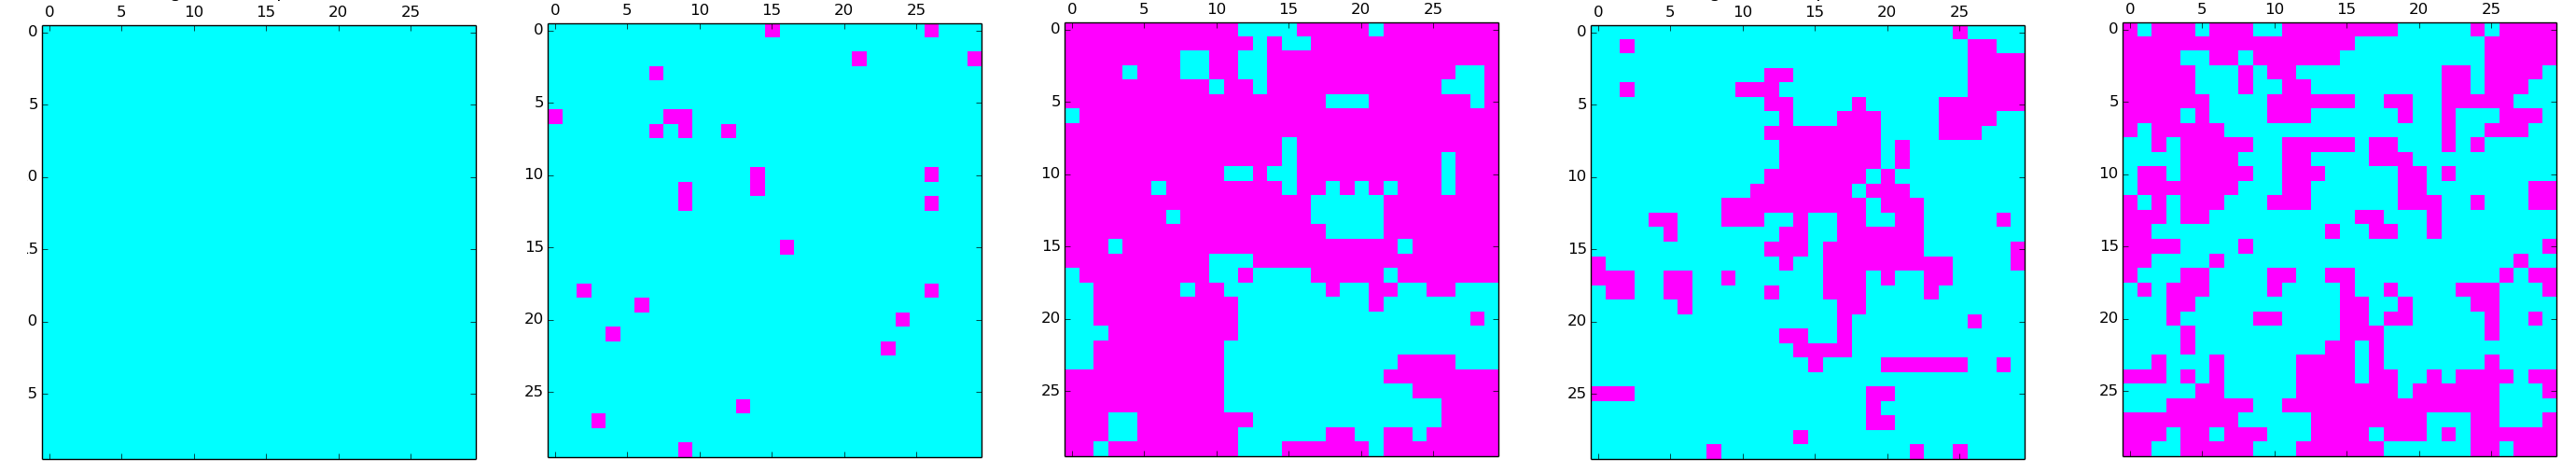
\includegraphics[scale=0.10]{pics/equilibrium_different_temperatures.png}
\caption{Equilibrium configuration for different dimensionless temperatures, $T$. Here a $30 \times 30$ lattice for $T$.  $T=1.0, 2.0, 2.2, 2.3, 3.0$. One can see the behavior of the system change close to the critical temperature where the phase transition happens. After the phase transition all magnetization is gone.} 
\label{fig:spin_neighbours}
\end{figure}


\subsection{Reproduction of results}

To see benchmark calculations along with programs used see:\\
\url{https://github.com/mulimoen/FYS3150CompPhy/}\\
Under the folder \emph{Project 4}.

\section{Conclusion}

\section{References}



\end{document}